\documentclass[aspectratio=169]{beamer}
%% For 4:3 aspect ratio:
%% \documentclass{beamer}
\usepackage{../git-course}

\title[git-course]{Exercises}
\author{Andrew Edwards \& Chris Grandin}
\date{\today}

\begin{document}
%% Needed to remove 'Figure:' from figure captions:
\setbeamertemplate{caption}{\raggedright\insertcaption\par}

\frame[plain]{
\titlepage
}

\section{Exercise 1}

\frame{\frametitle{Exercise 1 -- individuals}
  \bn
    \item Each person sets up a new repository \lstinline{***}, following \emph{git-course-intro.pdf}.
    \item Copy a text file (**we provide up front).
    \item Edit and commit and push....
    \item 
  \en
}


\section{Exercise 2}

\frame{\frametitle{Exercise 2 -- help from friends}
  \bn
    \item Consecutively number everyone 1, 2, 3, 4. Each group of four sitting together will collaborate.
    \item Person 1 will set up a new repository \lstinline{help-friends}, following \emph{git-course-intro.pdf}.
    \item Person 1 copies \lstinline{git-course/exercise-files/helpFriends.txt} into their new repository (on their computer).
    \item \lstinline{add}, \lstinline{commit}, \lstinline{push}. Check Network Graph.
    \item Persons 2, 3 and 4 then fork and clone the repository. 
    \item Everyone does a few edits on their paragraph (see \lstinline{helpFriends.txt}).
    \item \lstinline{commit} a few times, \lstinline{push}. Check Network Graph.
  \en
}

\frame{\frametitle{Exercise 2 -- help from friends}
  \bn
    \item Explore Network Graph (hover over the commits).
    \item Whoever is furthest behind (not that it matters), \lstinline{fetch} and \lstinline{merge} from the person who's furthest ahead (see \emph{git-course-intro.pdf}):
    \bi
      \item \lstinline{git remote add REMOTE-NAME REMOTE-URL}  (one time command)
      \item \lstinline{git fetch REMOTE-NAME}
      \item \lstinline{git merge REMOTE-NAME}
      \item \lstinline{git push}
      \item Check Network Graph (have to refresh).
      \item Check your collaborator's Network Graph (helpful if you care whether they have caught up with you).
    \ei
    \item Repeat step 2 until everyone is caught up.
    \item So if person A has fetch and merged person's B's work, person C can just fetch and merge from person A.
  \en
}





\end{document}

\section{Avoid}
\frame{\frametitle{Examples of what we can avoid}

  \centering
  \begin{figure}
    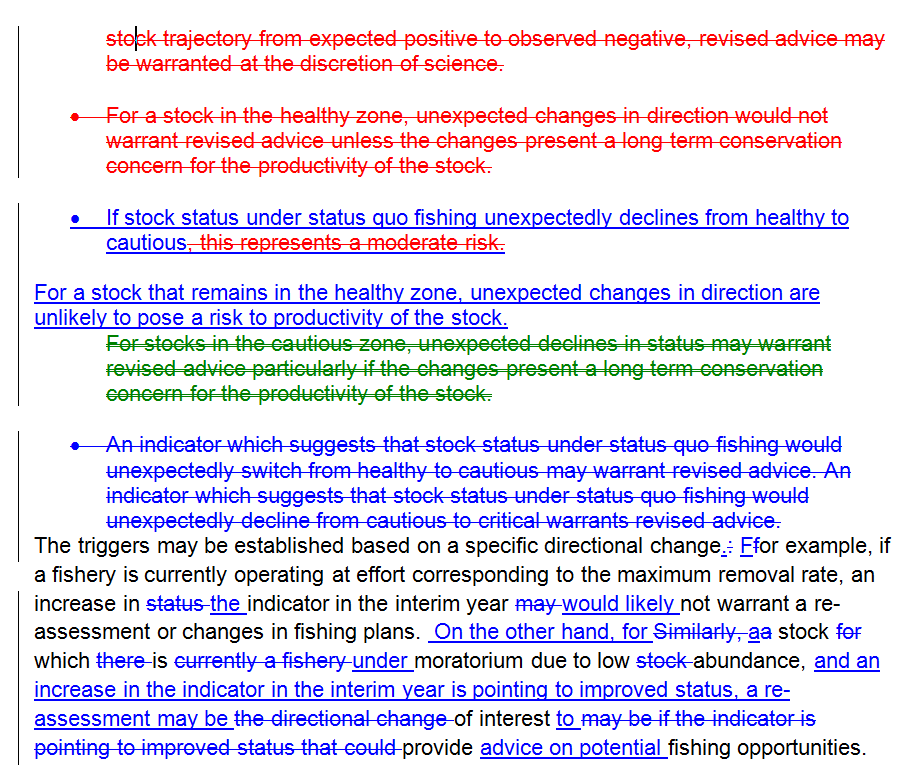
\includegraphics[
        width=\textwidth,
        height=0.8\textheight,
        keepaspectratio]
        {figures/interim.png}
  %\vspace{-3mm}
  %\caption{\tiny\url{https://www.reddit.com/user/NegativePitch}}
  \end{figure}
}

\frame{\frametitle{Relying on one person (e.g.~me) who holds up a project}

  Often we may be collaborating on a project but be busy on something else, yet our collaborator has time.

  \centering
  \begin{figure}
    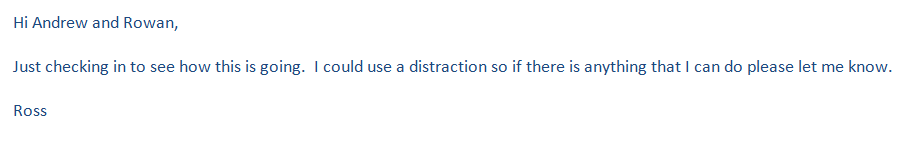
\includegraphics[
        width=\textwidth,
        height=0.8\textheight,
        keepaspectratio]
        {figures/procEmail.png}
  %\vspace{-3mm}
  %\caption{\tiny\url{https://www.reddit.com/user/NegativePitch}}
  \end{figure}
}

\frame{\frametitle{Cluttering up directories}

  We may want to keep old versions in case we have to go back, but then ...

  \centering
  \begin{figure}
    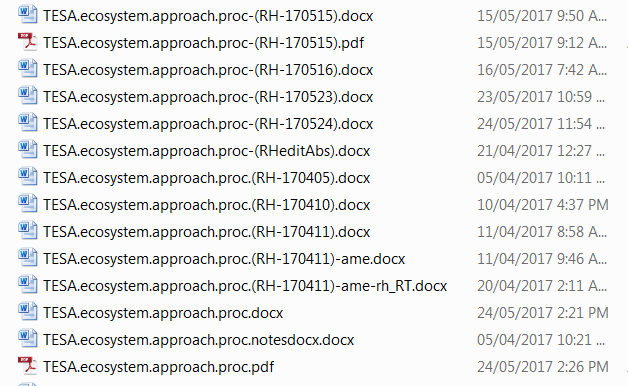
\includegraphics[
        width=\textwidth,
        height=0.8\textheight,
        keepaspectratio]
        {figures/EAversions.png}
  \end{figure}
}

\frame{\frametitle{Can work simultaneously on same document (and then merge)}

  Can all keep up with the latest version (checking and merging each other's work along the way), rather than ...

  \centering
  \begin{figure}
    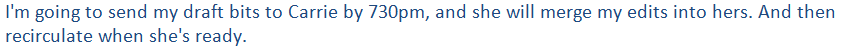
\includegraphics[
        width=\textwidth,
        height=0.8\textheight,
        keepaspectratio]
        {figures/proposalEmail.png}
  \end{figure}
}


\section{\gh\ advantages}

\frame{\frametitle{Can easily catch up with collaborator}

  Chris did a lot of work (`commits') from 11th May ...

  ~\\
  ~\\
  \includegraphics[
     width=\textwidth,
     height=0.6\textheight,
     keepaspectratio]
     {figures/netWorkGraph1}
}

\frame{\frametitle{Can easily catch up with collaborator}

  ... to 30th May:
  ~\\
  ~\\

  \includegraphics[
     width=\textwidth,
     height=0.6\textheight,
     keepaspectratio]
     {figures/netWorkGraph2}

  I did nothing in that time ... 

}

\frame{\frametitle{Can easily catch up with collaborator}

  ... but just needed three commands (that you'll learn) to get caught up:
  ~\\
  ~\\

  \includegraphics[
     width=\textwidth,
     height=0.6\textheight,
     keepaspectratio]
     {figures/netWorkGraph3}

  ~\\
  All files that Chris edited got updated, plus I now have any new files he created, and our folder structures are identical. 
}

\frame{\frametitle{Easy to answer other's questions}

  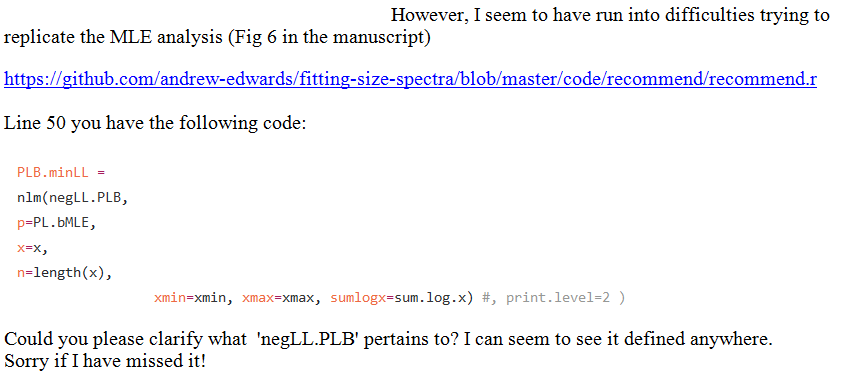
\includegraphics[
     width=\textwidth,
     height=0.80\textheight,
     keepaspectratio]
     {figures/MEEcodeQuest}


  Rather than go to the code on my laptop that I haven't looked at for six months, I could click on link and answer very quickly.
}

\frame{\frametitle{Easy to answer other's questions}

  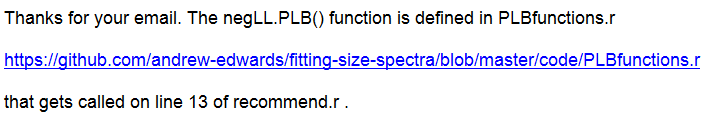
\includegraphics[
     width=\textwidth,
     height=0.80\textheight,
     keepaspectratio]
     {figures/MEEcodeAnswer}

~\\
  Can provide a clear answer with a link to the file I'm talking about. No ambiguity.
}



\frame{\frametitle{I wanted to check if I'd changed anything in the last month}

  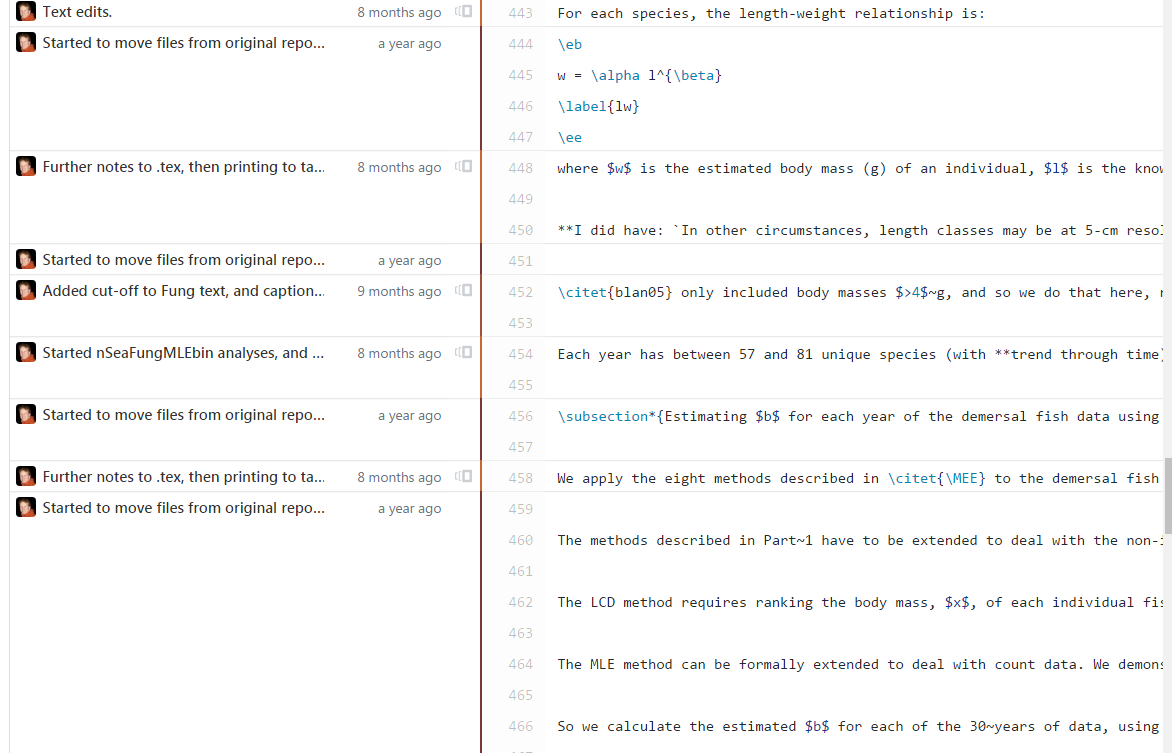
\includegraphics[
     width=\textwidth,
     height=0.80\textheight,
     keepaspectratio]
     {figures/history}

  I hadn't thought of that before [on \gh: Code -- $<$click file$>$ -- History].
}


\frame{\frametitle{Hake assessment}

  \bi 
    \item Collaboration between four/five US and Canadian scientists.
    \item Annual assessment.
    \item Full Bayesian statistical catch-at-age model (complex output).
    \item Short turnaround between getting final data and submitting assessment.
    \item Short turnaround between review meeting and publishing assessment (two days).
    \item 2015 and before -- lots of editing and amalgamating Word files late at night. 
  \ei
}

\frame{\frametitle{Hake assessment}
  \bi
    \item After running models we can now automatically generate full document, including all numbers, figures and tables (via knitr and latex, all shared on \gh).

    \item Was a lot of work in 2016 to set up, but 2017 was way less stressful and resulted in more polished document.
    \item Praise on Twitter from one of the reviewers!      
  \ei
  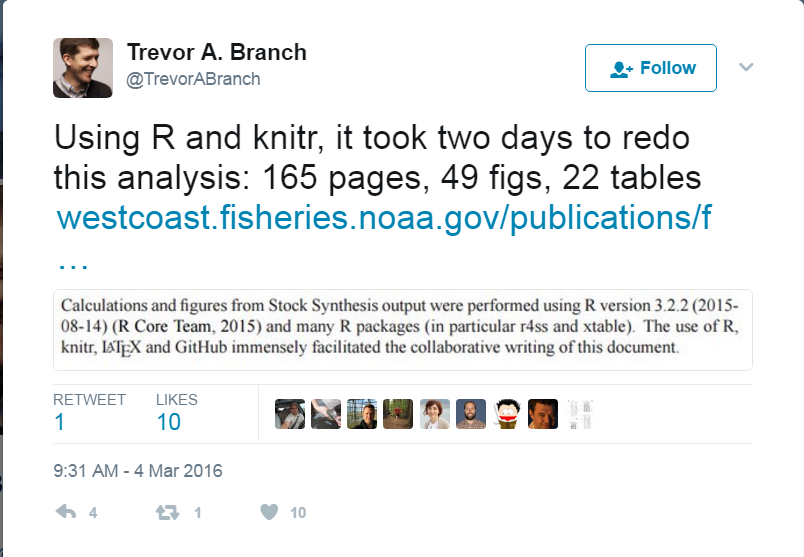
\includegraphics[
     width=\textwidth,
     height=0.50\textheight,
     keepaspectratio]
     {figures/trevorTweet}
}

\frame{\frametitle{Who wrote that piece of garbage?}

  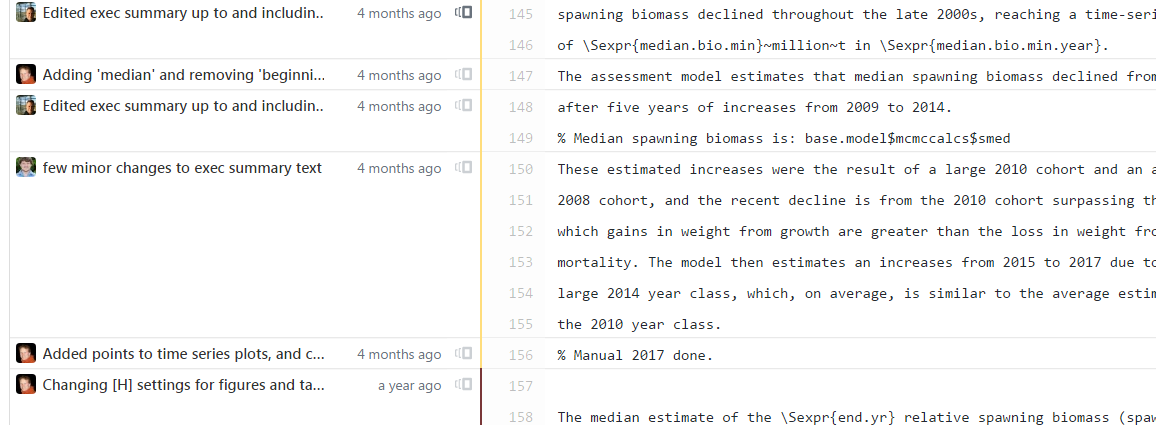
\includegraphics[
     width=\textwidth,
     height=0.80\textheight,
     keepaspectratio]
     {figures/blame}

~\\
  Can be useful [on \gh: Code -- $<$click file$>$ -- Blame].
}

\frame{\frametitle{Can properly keep track of (and discuss) issues}

Rather than lots of emails that get forgotten, the to-do list actually gets completed.

  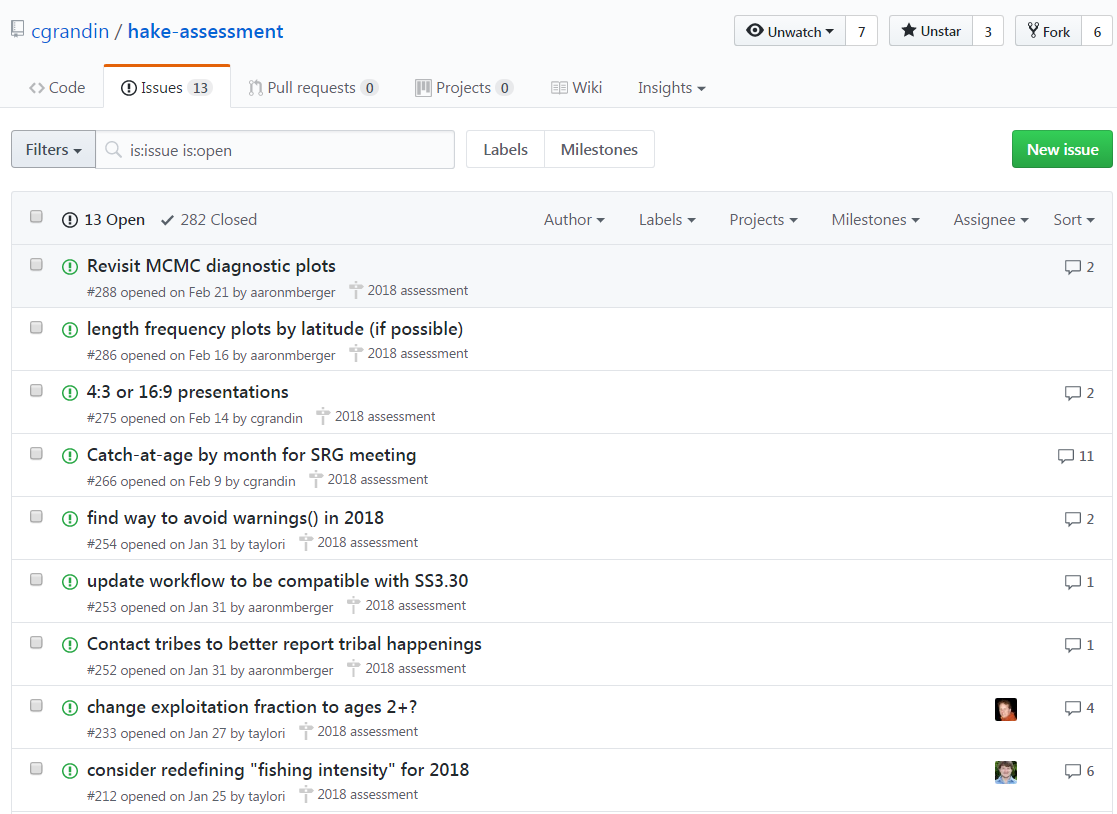
\includegraphics[
     width=\textwidth,
     height=0.80\textheight,
     keepaspectratio]
     {figures/hakeIssues}
}

\frame{\frametitle{Can properly keep track of (and discuss) issues}

And you don't have to follow up with co-authors (who do have it under control):

~\\
  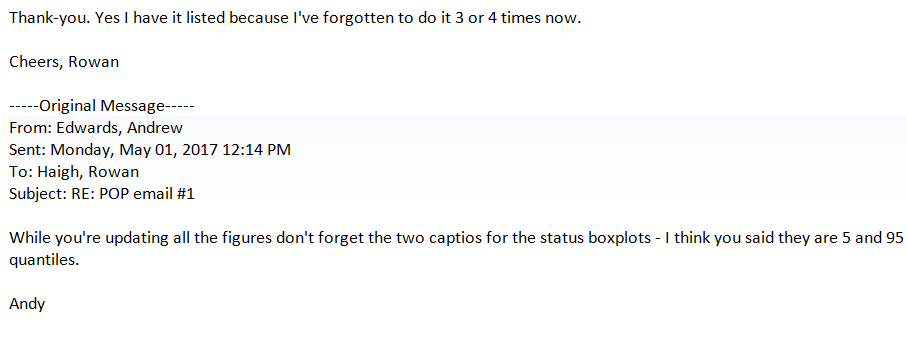
\includegraphics[
     width=\textwidth,
     height=0.80\textheight,
     keepaspectratio]
     {figures/captionEmail}
}


\section{Summary}

\frame{\frametitle{Summary}

  \bi
    \item Ideal for sharing of code.
    \item `Repositories' can be public or private.
    \item Caveat -- cannot (properly) collaborate on Word files. We will concentrate at first on just sharing code.
    \item Hake example is to show how far you can get.
    \item There is a learning curve, but once you use \gh\ you only really need a few main commands.
  \ei
}



\end{document}
